\section{Description}

% Summarize pair-HMMs. Brief, comment typically used but move onto FST right away
Statistical alignment is typically performed using pairwise hidden Markov
models (pair-HMMs).
% This computational machines consist of two output tapes and a set of states that
% emit symbols onto one or both tapes.
Pair-HMMs have the ability to rigorously model molecular sequence evolution and
can calculate the probability that two sequences are related, represented
$P(X, Y)$ \parencite{yoon_2009_hmm}.
However, a limitation of pair-HMMs is the ability to only model evolution of two
related sequences from an unknown ancestor.
Finite-state transducers (FSTs) have the ability to calculate the probability
that a sequence $Y$ evolved from sequence $X$, represented $P(Y | X)$.
FSTs share similar computational benefits as pair-HMMs in addition to well
established algorithms for combining them in different ways
\parencite{bradley2007transducers}.
A powerful and versatile algorithm is composition, which consists of sending the
output one FST as the input of a second FST.
The FST model implemented in COATi is designed by composing smaller FSTs, each
representing a specific process.

% Evolution FST
Pairwise alignment in COATi is implemented via the Evolution FST (Fig.
\ref{fig:evolution-fst}), based on existing transducers (e.g.
\cite{holmes2001evolutionary}).
This FST is formed by composing a substitution FST that encodes a 64x64 codon
model and an indel FST that models insertions and deletions, including frameshifts.
The innovation of the Evolution FST with respect to other transducers is the
combination of a codon substitution model with gaps that can occur at any
position of any length.

\begin{figure}[h!]
\begin{framed}
\centering
    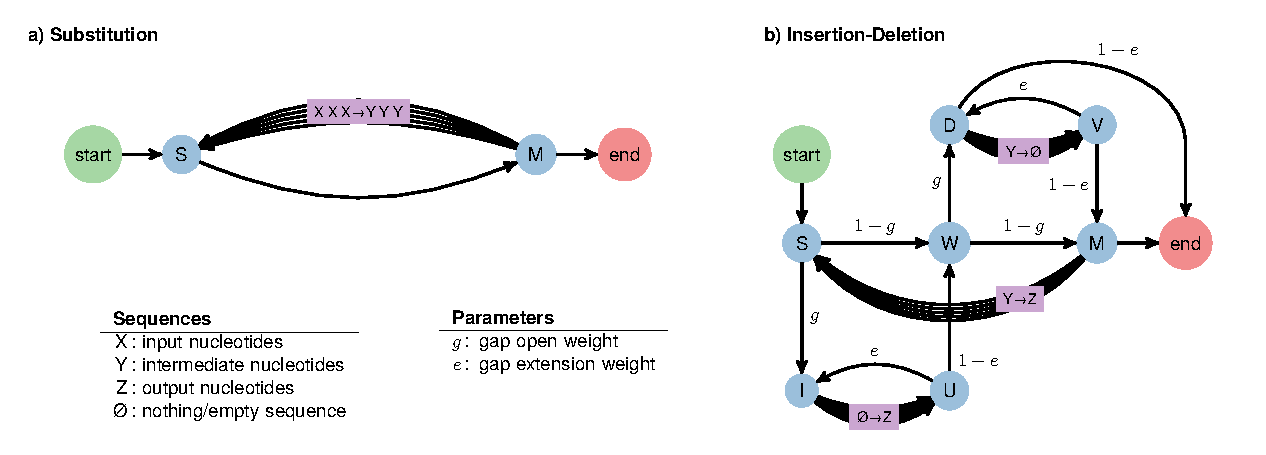
\includegraphics[width=\textwidth]{fig-evolution-fst.pdf}
    \caption{The evolution FST is assembled by composing a substitution FST and
    an indel FST. Each node represents a state in an FST while arcs display
    possible transitions between states (and their weights). Absorption and
    emission of symbols occurs between states. (a) The substitution FST
    encodes a 64x64 codon substitution model with 64 arcs from M to S. (b)
    The indel FST allows for insertions (I to U) and deletions (D to V).
    Contiguous insertions and deletions are always arranged for insertions to
    precede deletions to limit equivalent alignments.}
    \label{fig:evolution-fst}
\end{framed}
\end{figure}


% FST implementation
% A path through the FST that \green{results} from composing both sequences with
% the Evolution FST represent a pairwise alignment.
% To find the most \green{probable/likely} alignment we must find the shortest
% path through.
The alignment FST is the result from composing both sequences with the Evolution
FST.
Any path through the alignment FST represents a pairwise alignment, while the
shortest path corresponds to the best alignment.
However, composing large FSTs is an expensive operation and can be prohibitive.
Despite the existence of efficient C++ FST libraries (e.g. openFST
\cite{allauzen2007openfst}), runtime is still limiting for sequence pairs longer
than a few thousand nucleotides each.
To solve this issue, the search for an optimal path (alignment) can be
reformulated as a dynamic programming problem.
% Maintaining (or approximate??) the statistical framework, COATi implements a
% Gotoh-inspired algorithm thus reducing the problem to O(nm) runtime, n and m 
% length of sequences \green{citation?}

% Alignment itself?

% Evolution FST + Q matrix
% Marginal model? - Probably not
% DP - mention in a sentence or two.
% 1 figure: FST model? - results table?
